\chapter{Conclusion}

\section{Benchmarks}

A merge sort algorithm has been implemented in GPC for 80 million integers with a cutoff value 
of 2048. The actual sorting and merging is performed by the \texttt{MergeSort} kernel class
methods \texttt{MergeSort.serial\_ms} and \texttt{MergeSort.merge\_two}. The GPC code structures
how the Kernel tasks should interact and calls them in parallel. 

\lstinputlisting[style=myGPC]{code_samples/GPRM_MergeSort.gpc}
\overfullrule=2cm
This code is compiled into GPIR code by the compiler from the command line by entering \\
\texttt{gpcc GPRM\_MergeSort.gpc --threads=240} where the \texttt{threads} argument is an 
optional to manually adjust the number of total threads that are available to map tasks onto.

\newpage

\begin{figure}[!htb]
\pdfimageresolution=110
\centerline{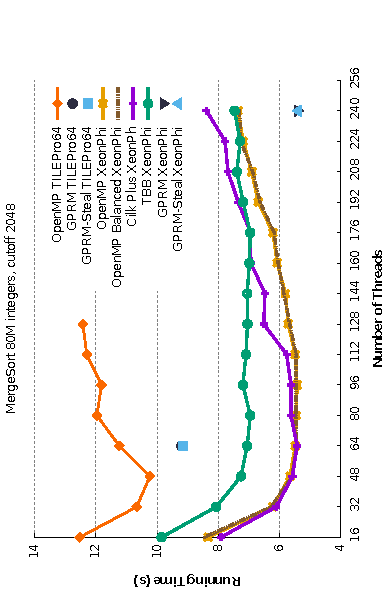
\includegraphics[angle=270, scale=1.3]{graphs/benchmark.pdf}}
\caption{Merge sort benchmarks for parallel frameworks \cite{GPRMBench}}
\label{fig:bench}
\end{figure}

The compiler compiles the merge sort GPC code into GPIR code identical to the GPIR code used to generate figure ~\ref{fig:bench}.
The \texttt{MergeSort} C++ Kernel class is also the same one used. From the figure it can easily be seen that the GPRM
far outperforms Cilk, TBB, and OpenMP on the XeonPhi, and OpenMp on the TILEPro64 for 240 threads in this specific example. 

Another thing to note is that the GPC code is a lot "nicer" than the code for the Cilk, TBB, and OpenMP
implementations, as it is almost completely pure C++.  It doesn't require the learning of how to use pragmas, 
or fork-join mechanisms.

\begin{figure}[!htb]
\pdfimageresolution=110
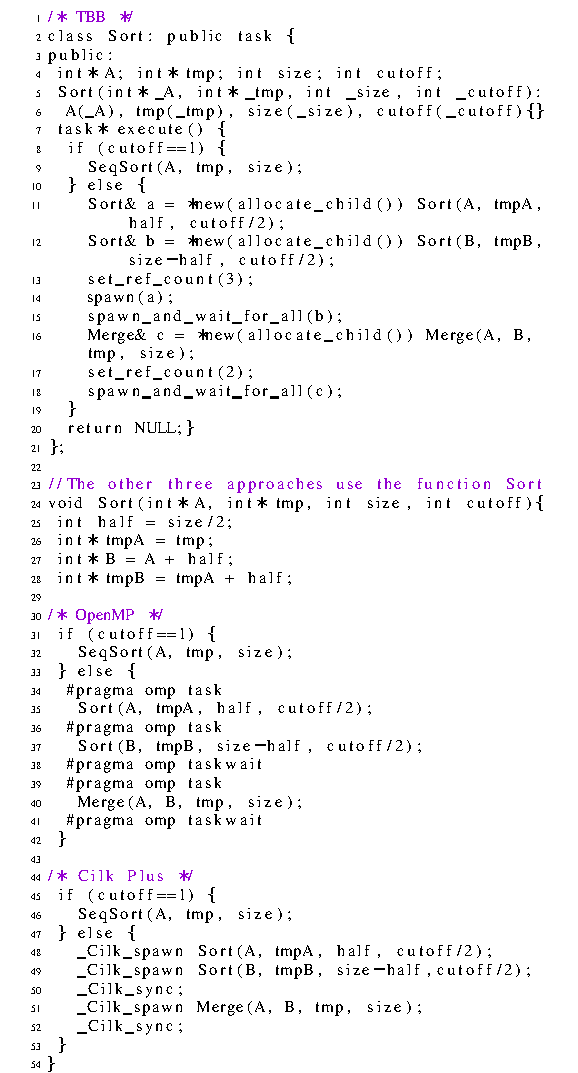
\includegraphics{graphs/merge.pdf}
\caption{Mergesort implementations in TBB, OpenMP, and CilkPlus \cite{GPRMBench}}
\end{figure}



\section{Summary}
The main goal of the project was to create a C-like language for the GPRM.
I believe that goal has been met as the language designed and implemented 
in this project is a purely functional parallel evaluation language which is an exact subset of C++ 
(apart from the two extra keywords). The language can be partially evaluated and compiled down to GPIR code 
which can be further compiled to be run on the GPRM. 

Methods and techniques that can be applied to interpret and partially evaluate purely
functional code have also been explored.

This project also leaves a lot of opportunities for future work. Compilers and Programming Languages in general have
multiple areas where there are constantly improvements to be made, most notably in language features and optimisations 
for code generation. A couple of possible improvements are explored in Chapter ~\ref{ch:future}.





